\subsection{Efficiencies}

 Detectors are not in 100\% of performance and the inefficiencies of detectors caused by hardware and software are needed to be evaluated corrected for cross section calculation. 

\subsubsection{Trigger Efficiency}

 There are mainly two aspects that determine the trigger efficiency~\cite{R_Bock}, one of which is the trigger algorithm designed to compromize between highly reducing background rate and keeping most of good events, and the other of which would be the dead time caused by electronics and performance of detectors involved in the trigger system. It is important to avoid double counting detectors' inefficiencies when evaluating trigger efficiencies. The definition of trigger efficiency genrally includes the inefficiency of scintillator counters and the formula is writtern as:

\begin{equation}
 \epsilon_{trigger\_eff} = \frac{PS1(3)\times N_{T1(3)}}{PS1(3) \times N_{T1(3)}+PS2(4)\times N_{T2(4)}},
 \label{trigger_eff}
\end{equation}

where $N_{T1(2,3,4)}$ is number of events triggered by T1(2,3,4) after prescaled by PS1(2,3,4). Tranditionally in Hall-A T1(3) is designed by requesting coincidence trigger signals between S1 and S2m, while T2(4) includes signals from GC in the trigger, which should carry the inefficiency effect of GC. However, during the E08014 experiment, T1(3) was modified to include GC signals in trigger, so the detection inefficiency of GC is canceled from the equation. Fig ~\ref{trig_eff} shows that the trigger efficiencies of our data on both arm were better than 99\%.

%\clearpage
\begin{figure}[h!]
\centerline{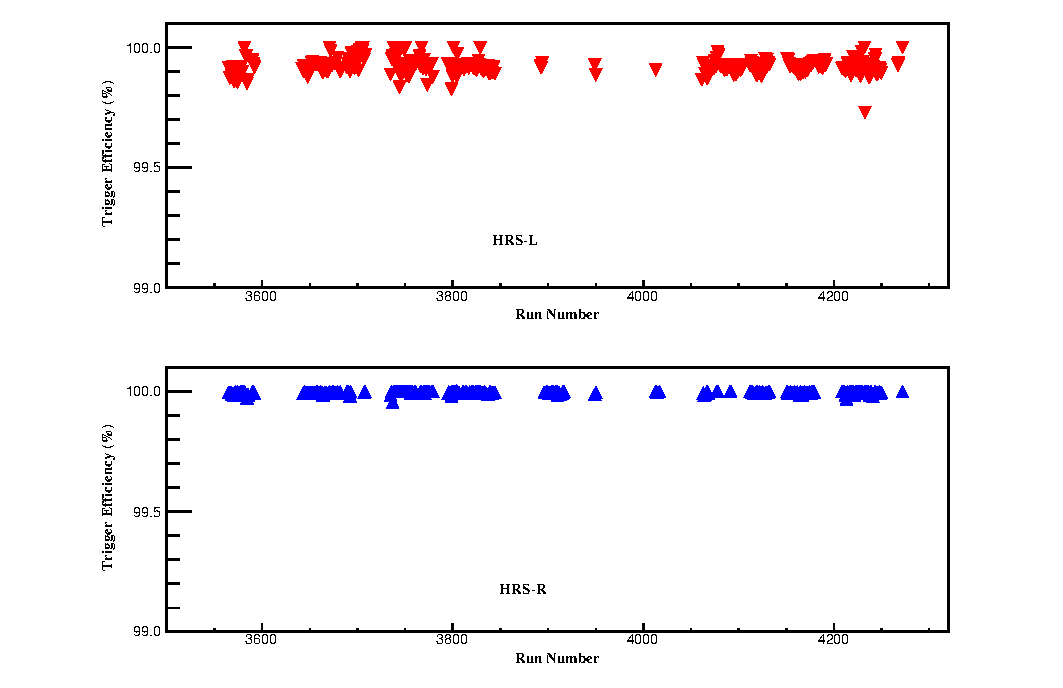
\includegraphics[width=0.7\linewidth]{figures/scin/Trigger_Eff.eps}}
\caption[Trigger Efficiencies]{\footnotesize{Trigger Efficiencies}}
\label{trig_eff}
\end{figure}

\subsubsection{One-Track Efficiency of VDCs}

Inefficiency of VDCs caused by hardware is neglectable and the majore source is from the misreconstruction of particle tracks during the tracking algorithm. Only one-track events are kept for analysis, and the good events threw away by zero-track and multi-tracks cut are corrected by the one-track efficiency defined as:

\begin{equation}
 \epsilon_{one\_track\_eff} = \frac{N_{Track=1}}{N_{0<=Tracks<=4}}
\end{equation}

 It is very important to select correct electron samples when calculating values of one-track efficiency. We need to avoid applying cuts on variables that require trakcing information, such as variables at focal plane and target plane, and cuting on other VDC variables will introduce other sources of inefficiencies. Cluster-reconstructed variables of calorimeters, such as E/P, can not be used when cutting electrons. cosmic ray events should also be removed since they come with big angles. We could not cut on TOF $\beta$ to suppress cosmic ray background due to the TDC multi-peaks issues on some scintillator bars. During the analysis, we used quasi-elastic carbon data which has low cosmic ray backgound due to the high rates,then applied cut on T1(3) trigger, GC ADC sum and Calorimeters ADC sum to select pure electron events, and we also require only one-hit on each scintillator bar for each event to remove events with multi-particles.From Table~\ref{vdc_table}, we obtained the fraction of one-track and multi-track events, which are above 99\% on each arm.

\begin{table}[h!]
\centering
\begin{tabular}{|c||ccccc|}
	\hline
\textbf{Number of tracks}  & 0 & 1 & 2 & 3 & 4     \\
	\hline \hline
HRS-L   & 0.0298\% & 99.1750\% & 0.7430\% & 0.0452\% & 0.0048\%  \\
        \hline
HRS-R   & 0.0482\% & 99.3600\% & 0.5446\% & 0.0388\% & 0.0073\%  \\
	\hline \hline
\end{tabular}
\caption{Fraction of different tracks events from quasi-elastic data,w/o $\beta$ cut}
\label{vdc_table}	
\end{table}



\subsubsection{Detection Efficiencies of PID detectors}
%\subsubsection{Gas Cherenkov}

For Gas Cherenkov detectors and lead-glass Calorimeters, there are two parts of informations needed to be extracted: the fractions of particles detected when they pass throught the detectors and leave signals, or called detection efficiencies; and the percentages of electrons remaining and pions contaiminating when applying PID cuts, also called PID-Cut efficiencies. PID-Cut efficiencies basically tangle with detection efficiencies due to the fact that we deal with detected events. We need to firstly evalute detection efficiencies and PID-Cut efficiencies will be discussed in next section. 

Detection efficiency of GC (Calorimeters) can be defined as:

\begin{equation}
 \epsilon_{detection\_eff}^{cer(calo)} = \frac{N_{detected}^{cer(calo)}}{N_{samples\_from\_calo(cer)}}
\end{equation}

where $N_{cer(calo)}$ is number of particles detected by GC (Calorimeters), and $N_{samples}$ is number of particle samples from Calorimeters (GC). During the analysis, we cut on T1(3) trigger and spectrometer acceptance, and pure electron were selected by applying cuts on main peaks of E/P spectra of Calorimeters when studying GC, or on the peaks of Cherenkov ADC Sum when studying Calorimeters. 

The design of Hall A Gas Cherenkov detectors should give high detection efficiency, since electrons can easily trigger the detectors with very low threshold, while pions and other particles from cosmic ray can not fire the detectors directly, and the inefficiency is caused by particles hitting the edges of gas boxes or PMT tubes. Fig ~\ref{cer_det_eff} shows that on both arm, the detection efficiencies of Gas Cherenkov detectors are close to 100\%.

%\clearpage
\begin{figure}[h!]
\centerline{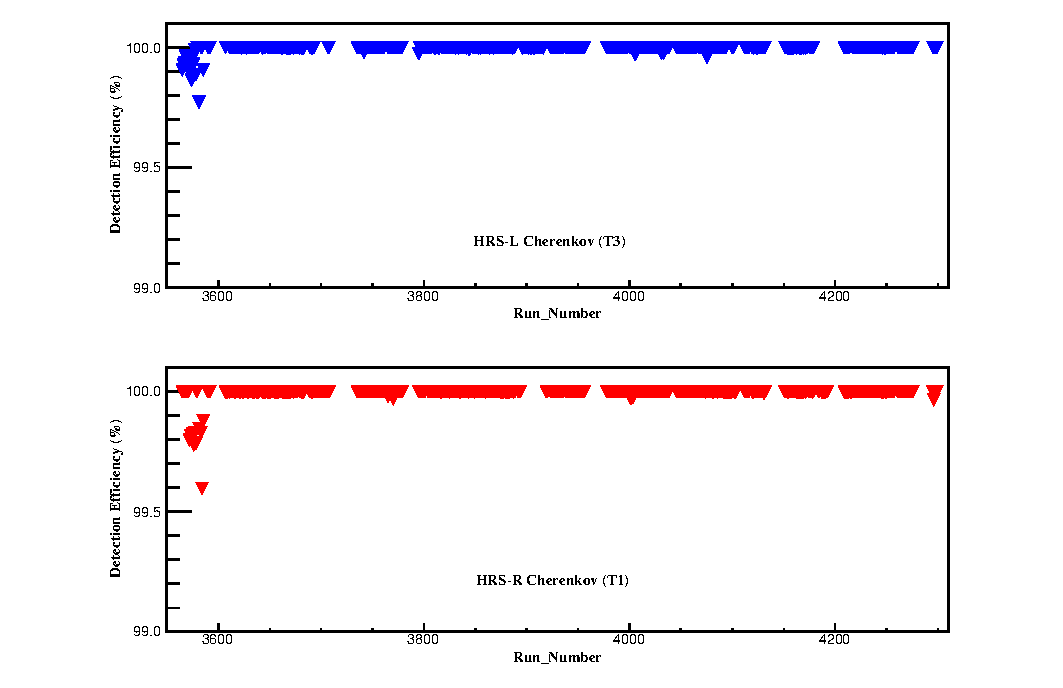
\includegraphics[width=0.7\linewidth]{figures/cer/Cer_Det_Eff.eps}}
\caption[Gas Cherenkov Detection Efficiency]{\footnotesize{Gas Cherenkov Detection Efficiency}}
\label{cer_det_eff}
\end{figure}

%\subsubsection{Calorimeters}
The detection efficiencies of lead glass calorimeters are expected to be lower than Gas Cherenkov detectors. Calorimeters are composed by piles of lead glass blocks, so the inefficiency of detection is mainly from particles going through gaps in between blocks or hitting the edges or PMT tubes before cascade. Cluster reconstruction when calculating deposited energy in lead glass blocks is another source of inefficiencies, especially when the electron rate is low and many low energy cosmic ray particles mix in.From Fig ~\ref{calo_det_eff}, we see that the detection efficiencies of calorimeters on both arm are still high than 99\% for most of runs, but for some runs with low electron rates, mainly for $^{3}He$ target with low beam current (Fig~\ref{calo_det_eff_mom}),the detection efficiencies are slightly lower, due to more cosmic ray contamination. Events from cosmic ray will eventually be removed by applying accpetance cuts and PID cuts, so no correction is necessary for those runs.  

\begin{figure}[h!]
 \centerline{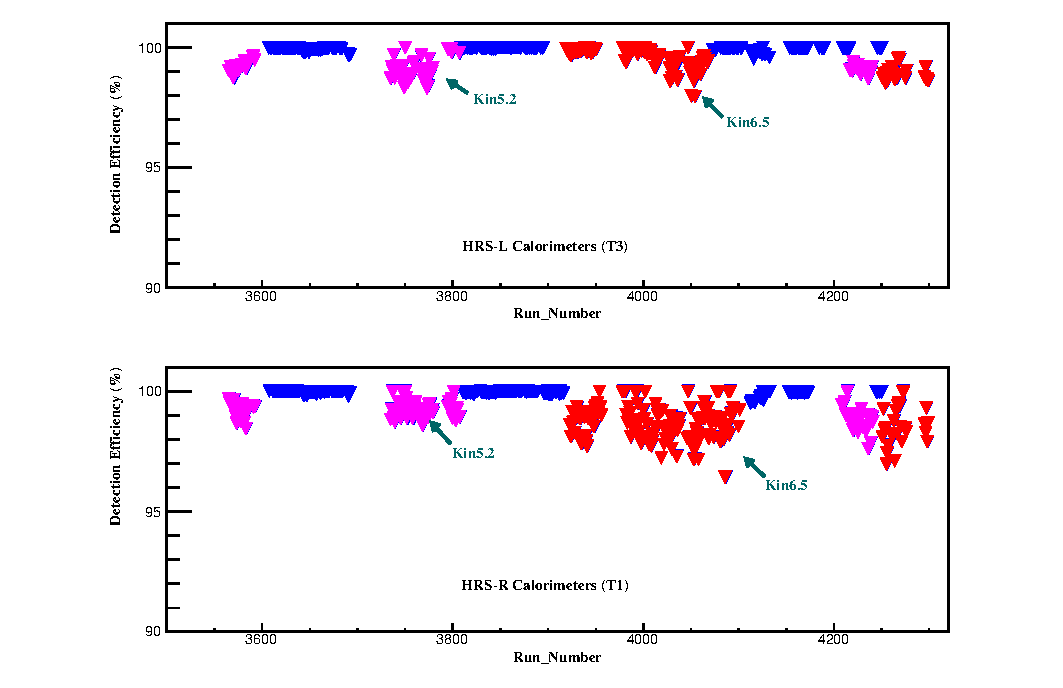
\includegraphics[width=0.7\linewidth]{figures/calo/Calo_Det_Eff1.eps}}
 \captionof{figure}{\footnotesize{Calorimeters: Efficiencies vs Run Number}}
 \label{calo_det_eff}
\end{figure}

\begin{figure}[h!]
 \centerline{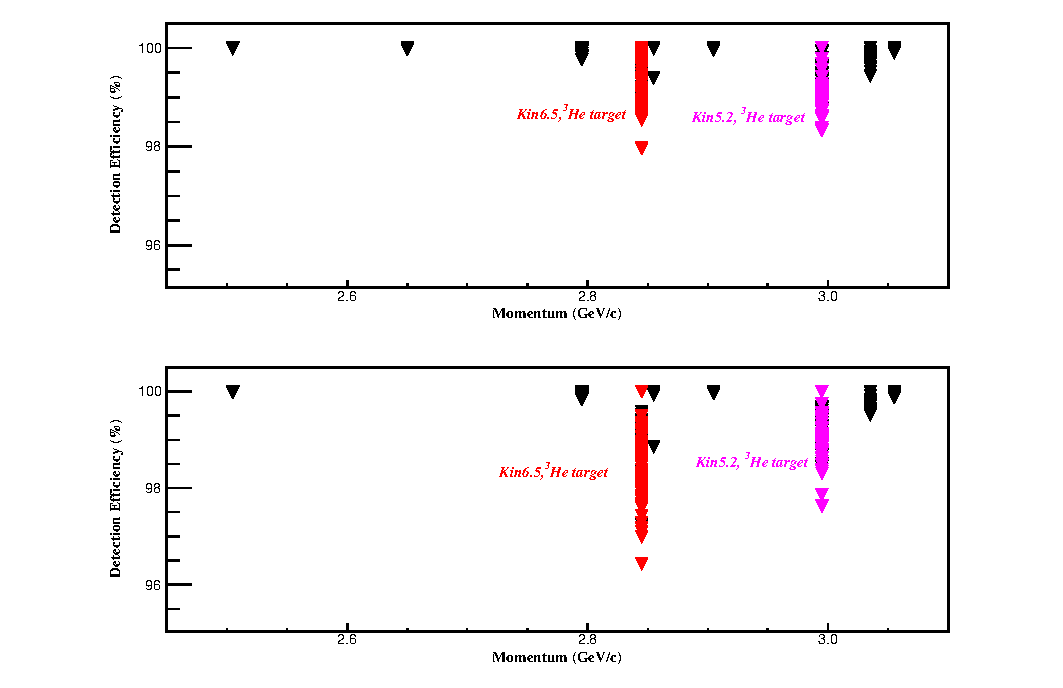
\includegraphics[width=0.7\linewidth]{figures/calo/Calo_Det_Eff_Mom1.eps}}
 \captionof{figure}{\footnotesize{Calorimeters: Efficiency vs Momentum}}
 \label{calo_det_eff_mom}
\end{figure}